\chapter{ORACLE APEX EXPRESS}

\section{Pengenalan Oracle Apex}
Application Express (Oracle Apex), dulu di sebut HTTP DB adalah sebuah Aplikasi database berbasis web yang digunakan dalam database Oracle. Oracle Apex ini mudah dipakai hanya menggunakan web browser saja dan proses pemrograman yang sederhana, serta mengembangkan ilmu dan kemampuan dengan Aplikasi ini secara aman dan cepat. Oracle Application Express memiliki kualitas database yang bagus, produktivitas dan standart luas yang dimiliki oleh perusahaan-perusahaan besar dan memiliki keamanan, stabilitas, ketersediaan dalam membangun suatu web. Application Express adalah suatu alat yang digunakan untuk membangun Aplikasi web-based. Selain itu Oracle Application Express tidak membutuhkan perangkat lainnya untuk mengembangkan, menyebarkan serta menjalankan Aplikasi, karena di dalam Oracle Application Express telah menyediakan tiga alat utama. Tiga alat utama ini memiliki Kegunaan yang penting di dalam Oracle Application Express:
\begin{enumerate}
    \item Application Builder : Membuat aplikasi, melihat aplikasi, mengimport aplikasi, mengatur service, mengatur user aplikasi dan memantau aktifitas yang di lakukan pengguna.
    \item SQL Workshop : Membuat tabel dan komponennya (menggunakan kode PL-SQL secara manual maupun otomatis), melihat struktur tabel dan komponennya, mengimpor dan mengekspor script.
    \item Utilitas : melihat report table dan komponennya dan history aplikasi.
\end{enumerate}
\section{Jenis Aplikasi yang dapat dibuat dengan Application Express}
Aplikasi Express digunakan untuk Aplikasi yang membuat report data pada database. Report data dapat berupa report text yang dikaitkan dengan report lainnya dan grafik supaya lebih efektif. Application Express juga bisa digunakan dalam pengeditan database meskipun memiliki kapasitas yang besar. Banyak bentuk tampilan yang bisa dibuat menggunakan Application Express antara lain: radio group,checkboxes, select list, shuttles, text editor dan date pickers. 
\section{Langkah Langkah Membuat Aplikasi Akademik Sederhana}

Dalam pembuatan aplikasi akademik sederhana, kita harus memimiliki data pada microsoft excel, dan harus sudah kita normalisasikan. Normalisasi adalah proses pengelompokkan atribut data yang membentuh sebuah entitas sederhana, tidak redudansi, dan fleksibel. Sehingga dapat dipastikan bahwa database yang akan kita buat berkualitas baik. Tujuan normalisasi itu sendiri yaitu untuk menghilangkan dan mengurangi adanya redudansi data dan memastikan depensi data (data berada pada tabel yang tepat). 
\begin{enumerate}
    \item Langkah pertama, kita harus membuka microsoft excel dan membuat data yang sudah kita normalisasikan seperti gambar dibawah ini
    \begin{figure}[!htbp]
    \begin{center}
    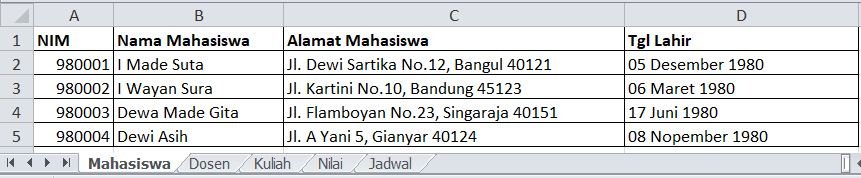
\includegraphics[scale=0.9]{section/ica51.JPG}
    \caption{Tampilan Tabel Mahasiswa}
    \end{center}   
    \end{figure} 
    
    \begin{figure}[!htbp]
    \begin{center}
    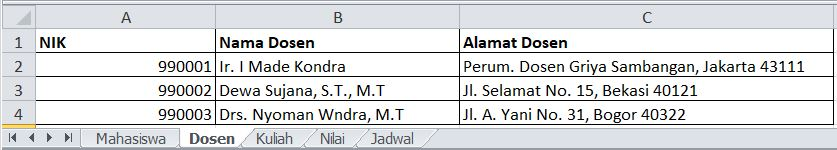
\includegraphics[scale=0.9]{section/ica52.JPG}
    \caption{Tampilan Tabel Dosen}
    \end{center}   
    \end{figure} 
    
    \begin{figure}[!htbp]
    \begin{center}
    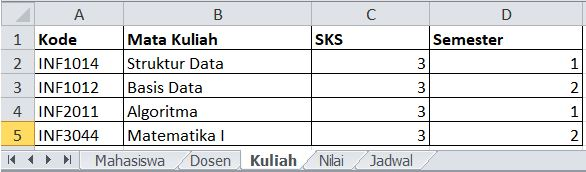
\includegraphics[scale=0.9]{section/ica53.JPG}
    \caption{Tampilan Tabel Kuliah}
    \end{center}   
    \end{figure} 

    \begin{figure}[!htbp]
    \begin{center}
    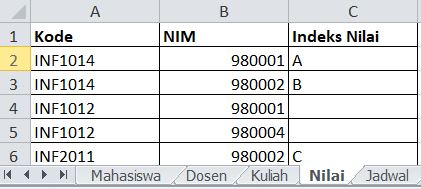
\includegraphics[scale=0.9]{section/ica54.JPG}
    \caption{Tampilan Tabel Nilai}
    \end{center}   
    \end{figure} 
    
    \begin{figure}[!htbp]
    \begin{center}
    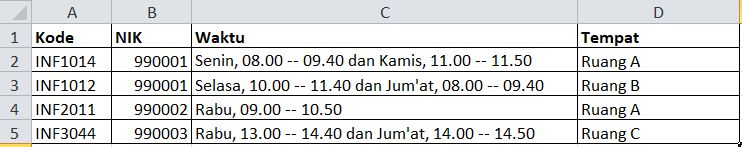
\includegraphics[scale=0.9]{section/ica55.JPG}
    \caption{Tampilan Tabel Jadwal}
    \end{center}   
    \end{figure} \vspace{3cm}
    
    \item Setelah data dibuat, kita Login dengan workspace seperti gambar dibawah ini
    \begin{figure}[!htbp]
    \begin{center}
    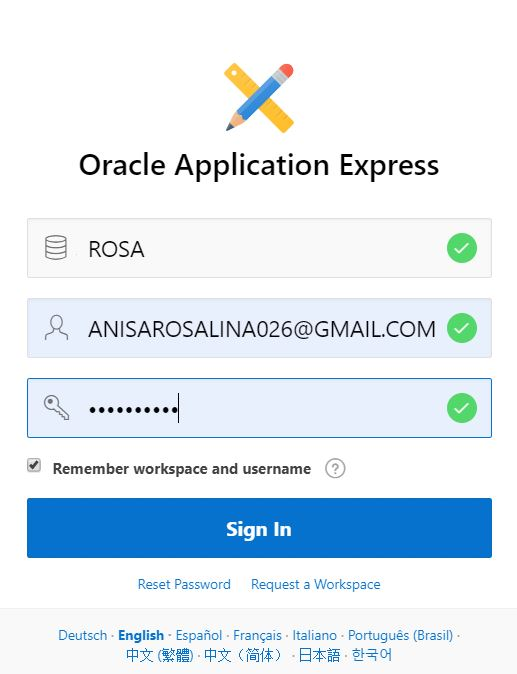
\includegraphics[scale=0.9]{section/ica27.JPG}
    \caption{Login dengan workspace}
    \end{center}   
    \end{figure} \vspace{12cm}
\item Setelah itu Klik application builder, Maka akan muncul tampilan seperti di bawah.
    \begin{figure}[!htbp]
    \begin{center}
    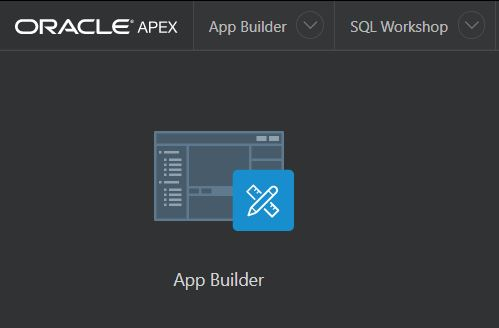
\includegraphics[scale=0.9]{section/ica29.JPG}
    \caption{Tampilan Halaman App Builder}
    \end{center}   
    \end{figure} 
\item Lalu Klik create seperti gambar dibawah ini
    \begin{figure}[!htbp]
    \begin{center}
    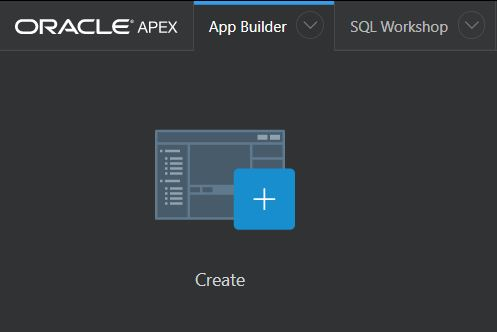
\includegraphics[scale=0.9]{section/ica30.JPG}
    \caption{Tampilan Halaman Create}
    \end{center}   
    \end{figure} \vspace{6cm}
\item Kemudian klik Next from a file
    \begin{figure}[!htbp]
    \begin{center}
    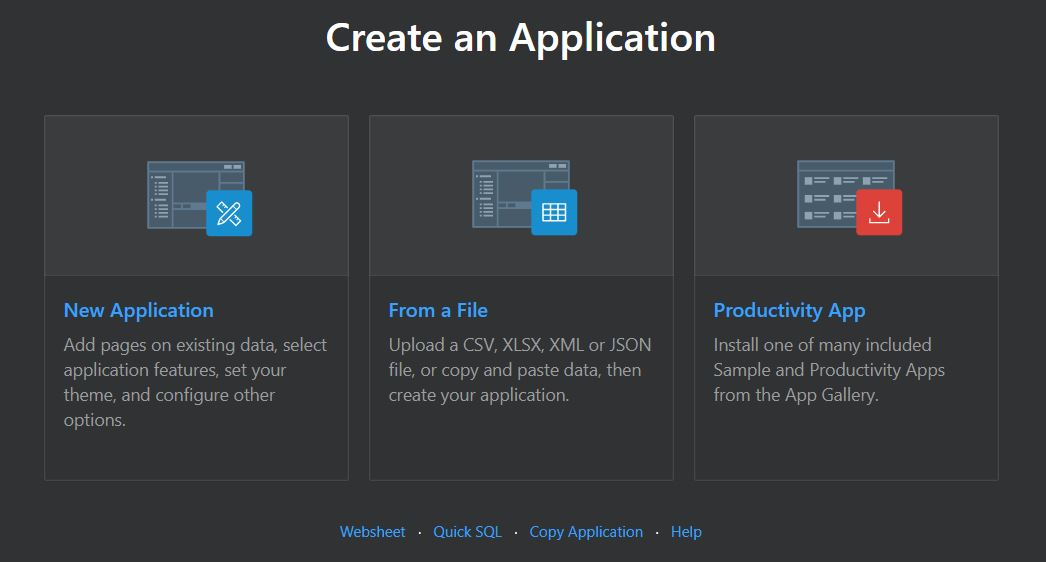
\includegraphics[scale=0.7]{section/ica31.JPG}
    \caption{Tampilan Halaman Create an Application}
    \end{center}   
    \end{figure} 
\item Langkah selanjutnya yaitu pilih choose file, dan pilih file yang akan kita buat
    \begin{figure}[!htbp]
    \begin{center}
    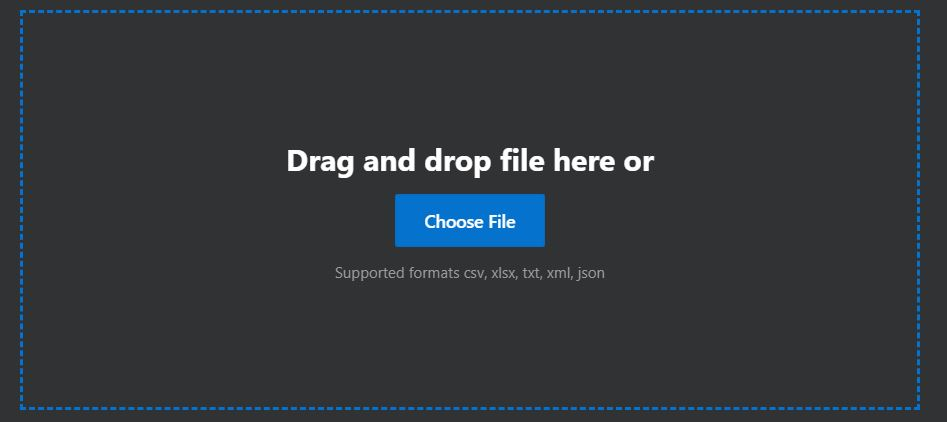
\includegraphics[scale=0.7]{section/ica32.JPG}
    \caption{Tampilan Halaman Choose File}
    \end{center}   
    \end{figure} \vspace{6cm}
\item Masuk ke table name lalu isi Mahasiswa, dan Select Sheet pilih mahasiswa sesuaikan apa yang tadi kita buat. karena yang pertama akan kita buat adalah tabel mahasiswa. setelah selesai lalu buat lagi tabel Dosen, Kuliah, Nilai dan Jadwal begitu juga dengan Select Sheet nya.
    \begin{figure}[!htbp]
    \begin{center}
    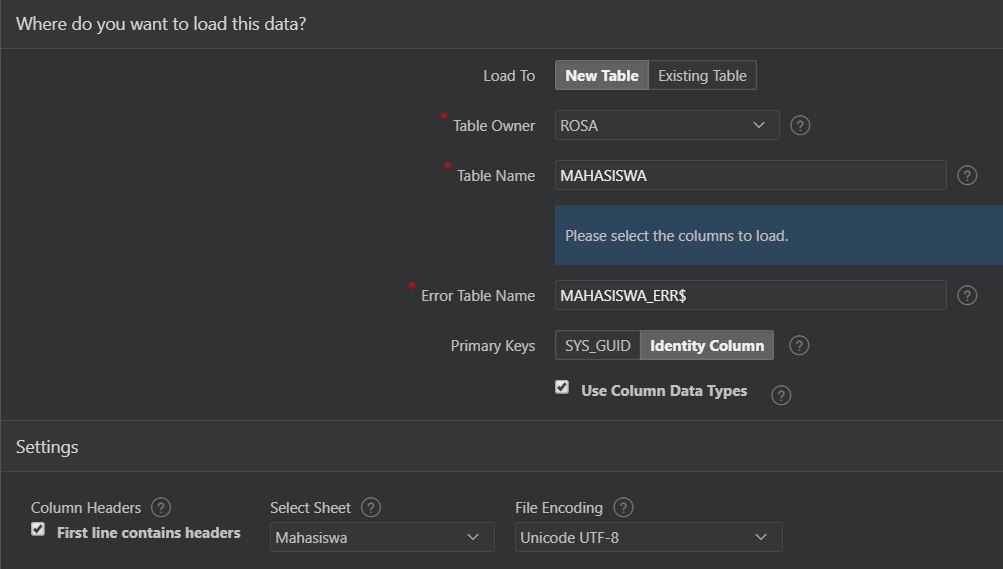
\includegraphics[scale=0.7]{section/ica41.JPG}
    \caption{Tampilan Halaman Pengisian Name Table dan Select Sheet}
    \end{center}   
    \end{figure} 
    
\item Ketika Tabel mahasiswa telah dibuat lalu klik load data lalu close, dan lanjutkan pembuatan tabel dosen, kuliah, nilai dan jadwal.
    \begin{figure}[!htbp]
    \begin{center}
    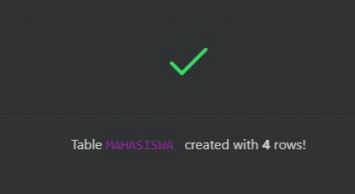
\includegraphics[scale=0.9]{section/ica56.JPG}
    \caption{Tampilan Halaman Tabel Mahasiswa telah Berhasil}
    \end{center}   
    \end{figure} \vspace{6cm}
    
\item Tabel yang tadi kita buat, bisa dilihat dengan cara kita klik SQL Workshop seperti gambar dibawah ini
    \begin{figure}[!htbp]
    \begin{center}
    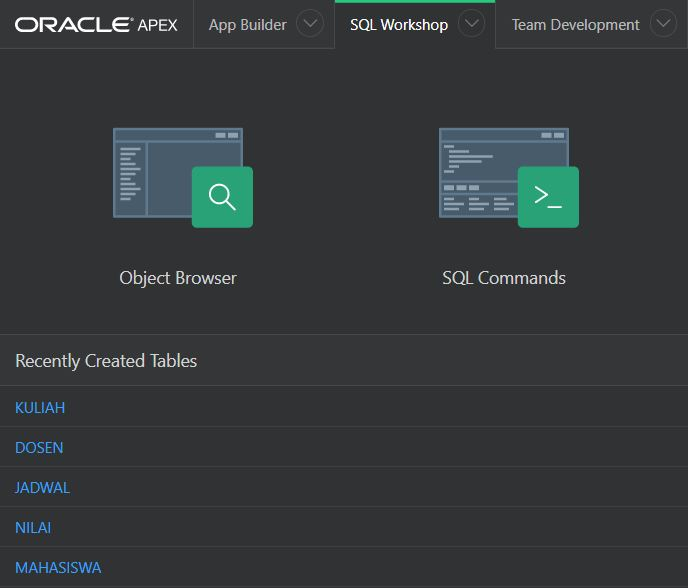
\includegraphics[scale=0.9]{section/ica57.JPG}
    \caption{Tampilan Halaman SQL Workshop}
    \end{center}   
    \end{figure} 
    
\item Langkah selanjutnya kita klik tabel mahasiswa sebagai contohnya
    \begin{figure}[!htbp]
    \begin{center}
    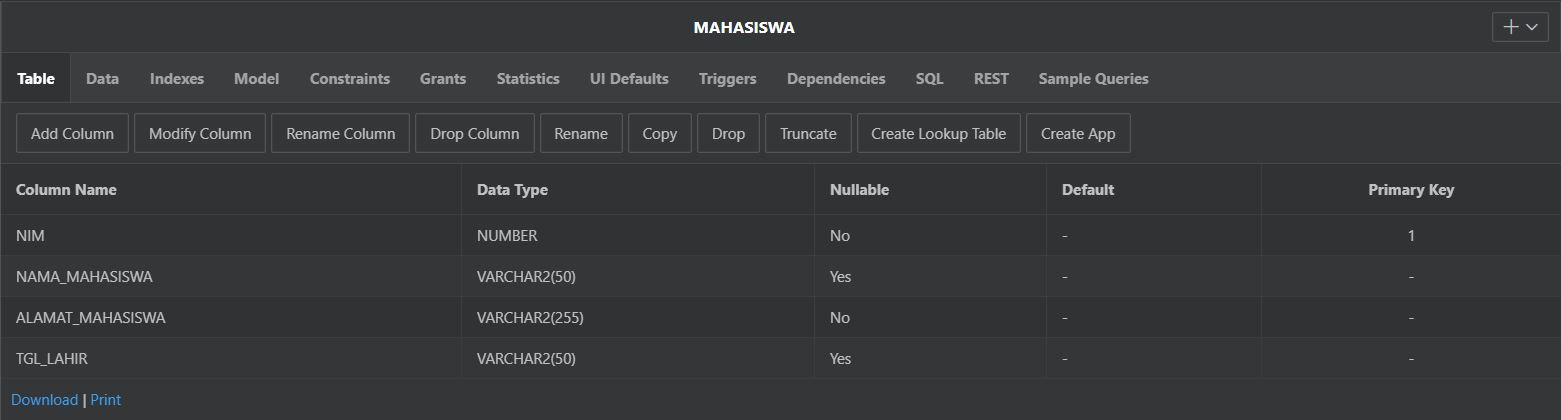
\includegraphics[scale=0.4]{section/ica58.JPG}
    \caption{Tampilan Halaman Mahasiswa}
    \end{center}   
    \end{figure} \vspace{5cm}

\item Klik Mahasiswa lalu klik  Modify Column
    \begin{figure}[!htbp]
    \begin{center}
    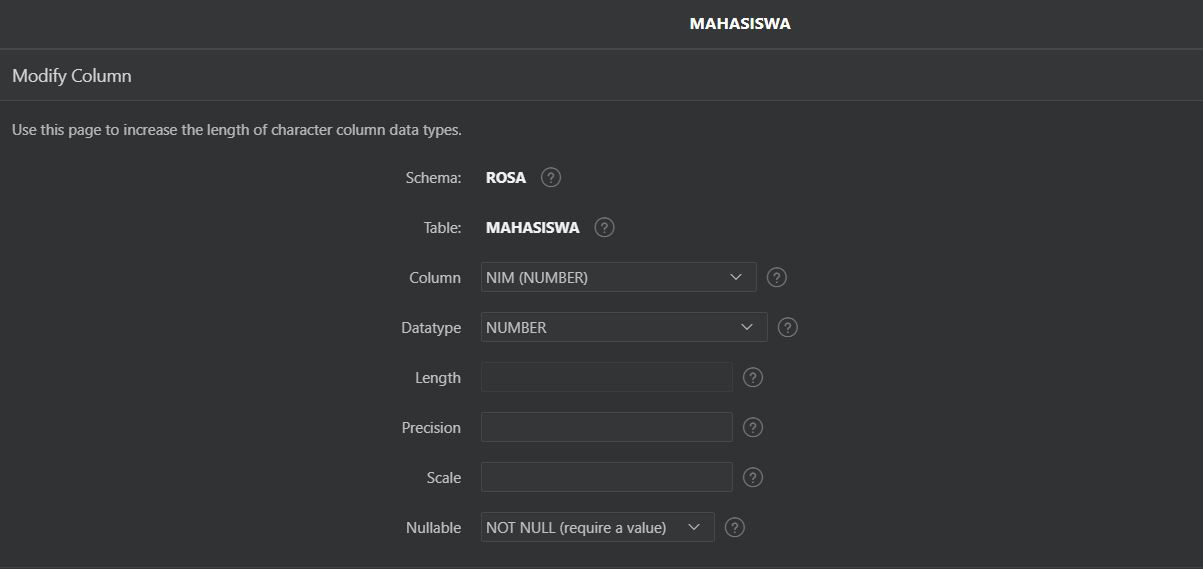
\includegraphics[scale=0.6]{section/ica60.JPG}
    \caption{Tampilan Halaman Tabel Mahasiswa}
    \end{center}   
    \end{figure} 
    
\item Pilih Dosen - Contrains - Create adalah cara untuk membuat primary key, dan foreign key 
    \begin{figure}[!htbp]
    \begin{center}
    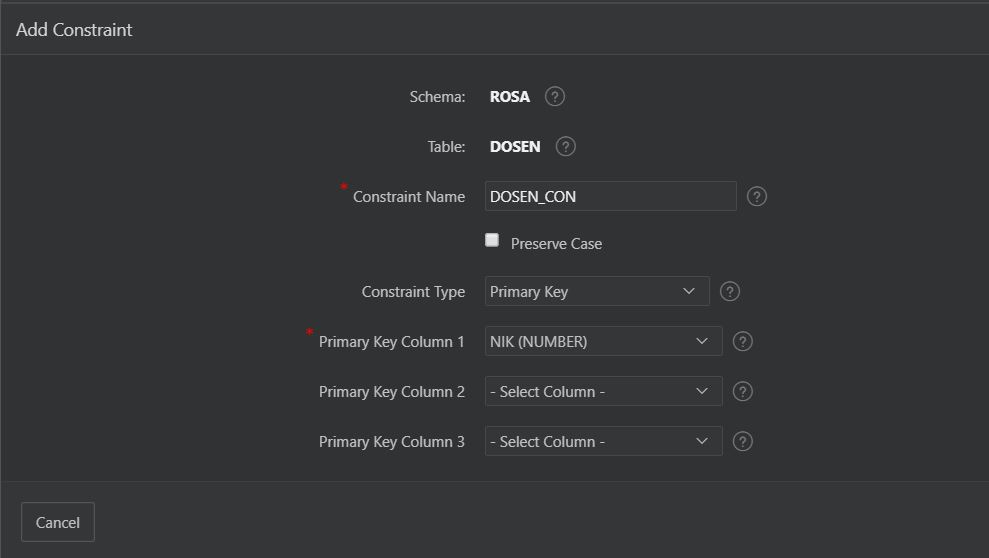
\includegraphics[scale=0.7]{section/ica1.JPG}
    \caption{Tampilan Halaman Tabel Dosen}
    \end{center}   
    \end{figure} 

\item Kemudian pilih tabel Jadwal - Clik Constrains - create pilih foreign key lalu klik  kode dan klik NIK. 
    \begin{figure}[!htbp]
    \begin{center}
    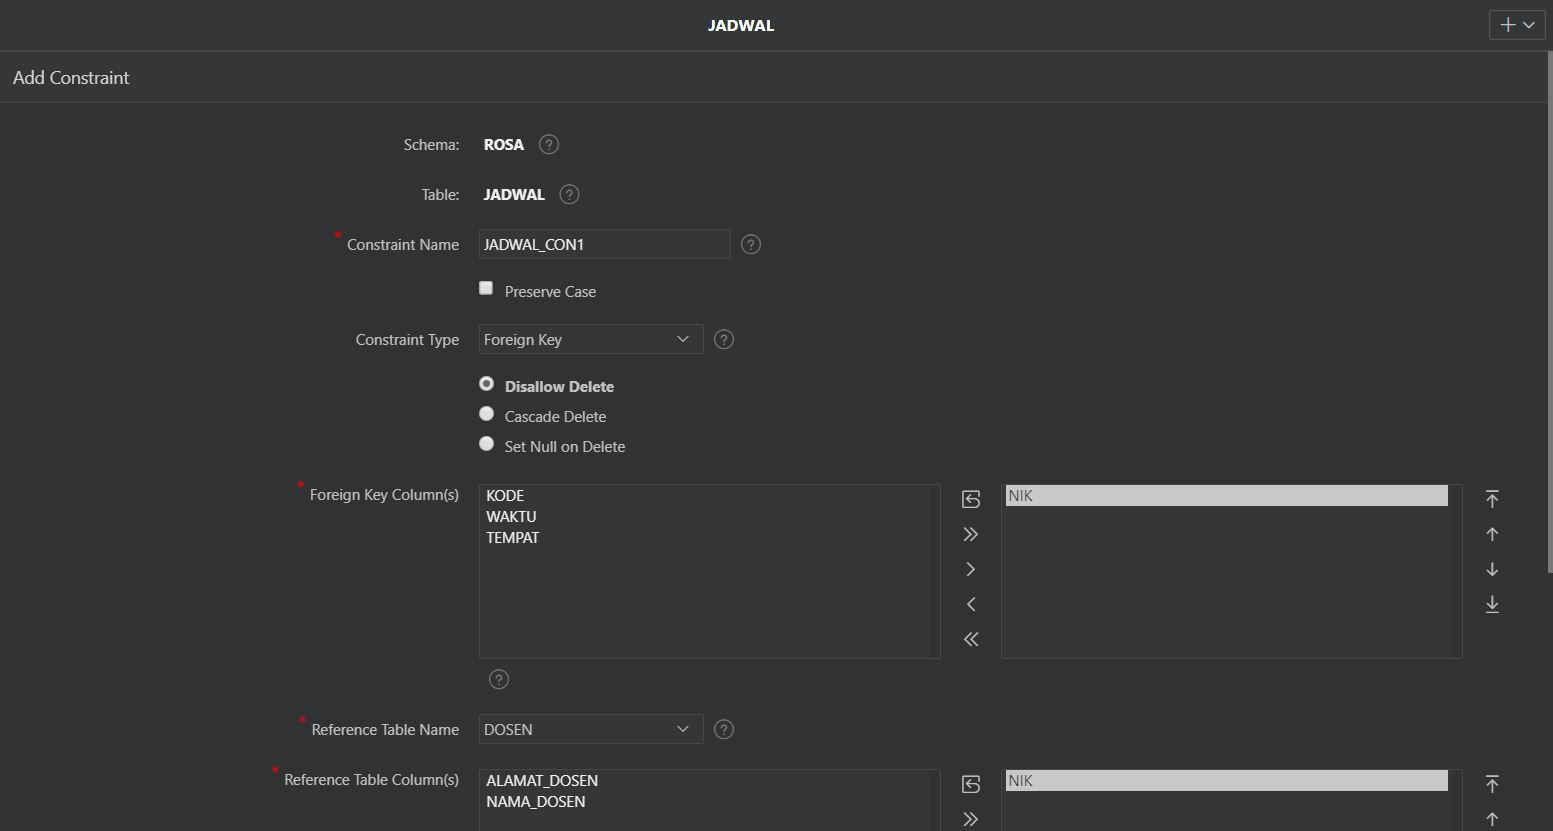
\includegraphics[scale=0.4]{section/ica7.JPG}
    \caption{Tampilan Halaman Tabel Jadwal}
    \end{center}   
    \end{figure} 
    
\item Setelah itu, Klik New Application kemudian buat nama aplikasinya, Aplikasi Akademik Sederhana.`
    \begin{figure}[!htbp]
    \begin{center}
    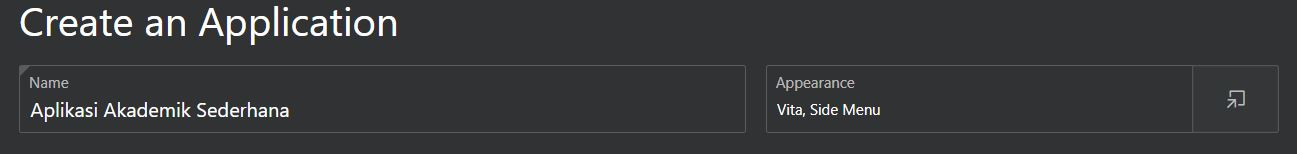
\includegraphics[scale=0.5]{section/ica38.JPG}
    \caption{Tampilan Halaman Add Page}
    \end{center}   
    \end{figure} 

\item Kita sudah akan membuat nama Aplikasi Akademik Sederhana,Setelah itu pilih add page yang didalamnya terdapat :
\begin{enumerate}
    \item Blank
    \item Calendar
    \item Cards
    \item Chart
    \item Dashboard
    \item Faceted Search
    \item Form
    \item Interactive Grid
    \item Interactive Report
    \item Master Detail
    \item Wizard
    \item Multiple Reports
\end{enumerate}
Untuk mengambil contoh, Saya memilih interaktive report, master detail, dan cards page.  
    \begin{figure}[!htbp]
    \begin{center}
    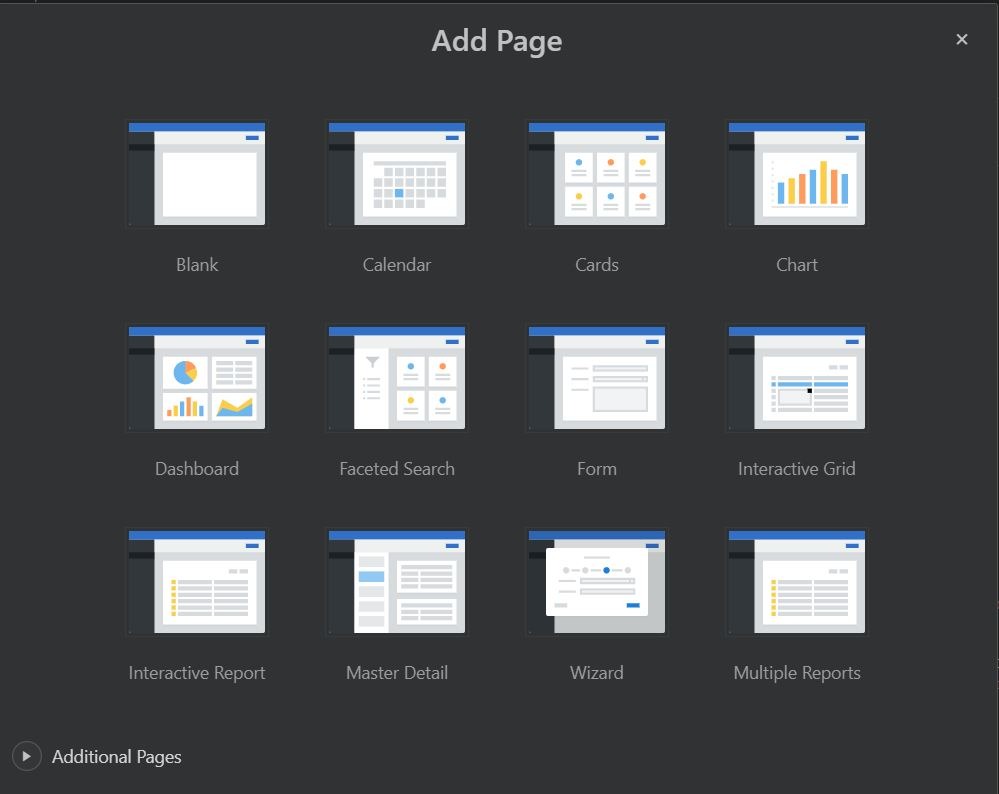
\includegraphics[scale=0.6]{section/ica20.JPG}
    \caption{Tampilan Halaman Add Page}
    \end{center}   
    \end{figure} \vspace{8cm}

\item Setelah itu pilih interaktive report, dan Berinama tabel KULIAH seperti gambar dibawah ini. Begitu juga dengan Dosen, Mahasiswa, Nilai dan Jadwal.
    \begin{figure}[!htbp]
    \begin{center}
    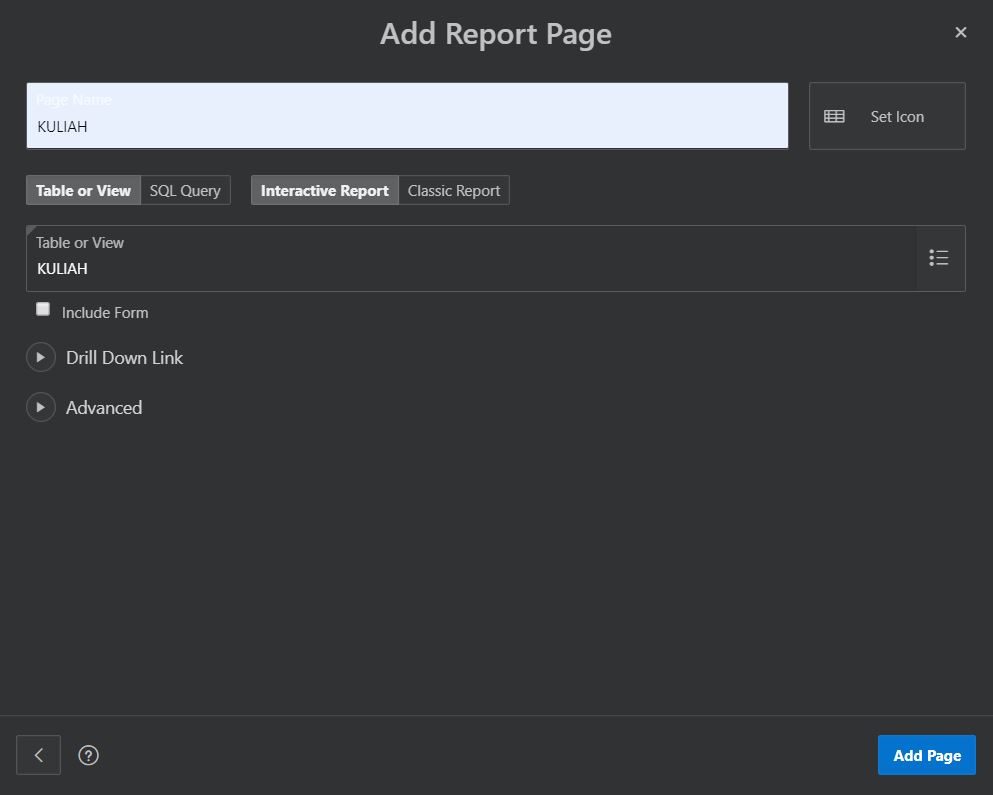
\includegraphics[scale=0.6]{section/ICA25.JPG}
    \caption{Tampilan Halaman interaktive report}
    \end{center}   
    \end{figure}  
\item Kemudian pilih Master detail, dan berinama tabel MAHASISWA seperti gambar dibawah ini. Master detail hanya saya buat 2 yaitu DOSEN Dan MAHASISWA. \vspace{8cm}
    \begin{figure}[!htbp]
    \begin{center}
    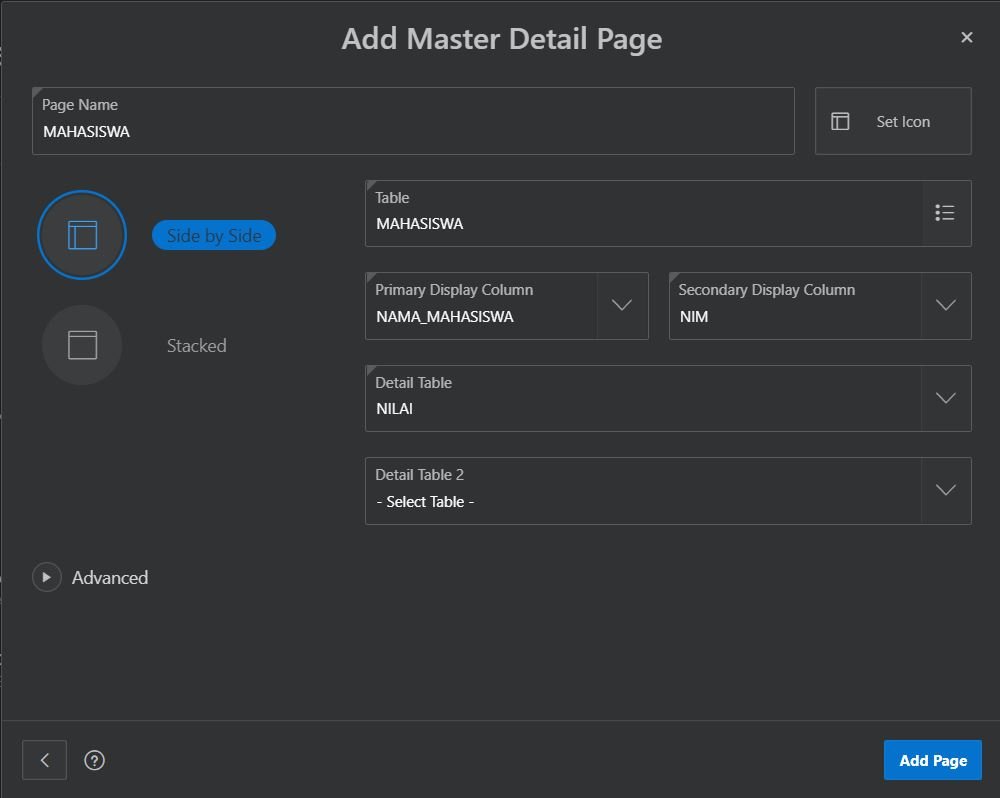
\includegraphics[scale=0.5]{section/ICA21.JPG}
    \caption{Tampilan Halaman Master Detail}
    \end{center}   
    \end{figure} 
\item Kemudian pilih Cards, dan berinama tabel MAHASISWA seperti gambar dibawah ini. Cards hanya saya buat 2 yaitu DOSEN Dan MAHASISWA.
    \begin{figure}[!htbp]
    \begin{center}
    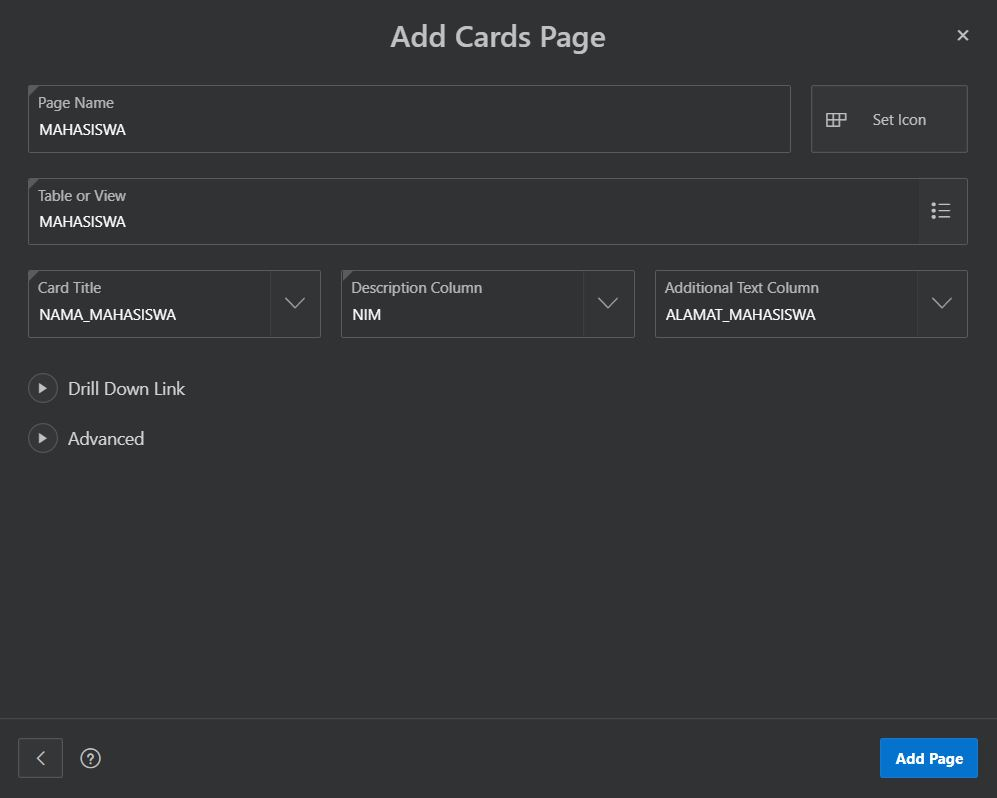
\includegraphics[scale=0.5]{section/ICA44.JPG}
    \caption{Tampilan Halaman Cards}
    \end{center}   
    \end{figure} 
\item Page yang telah kita buat tadi
    \begin{figure}[!htbp]
    \begin{center}
    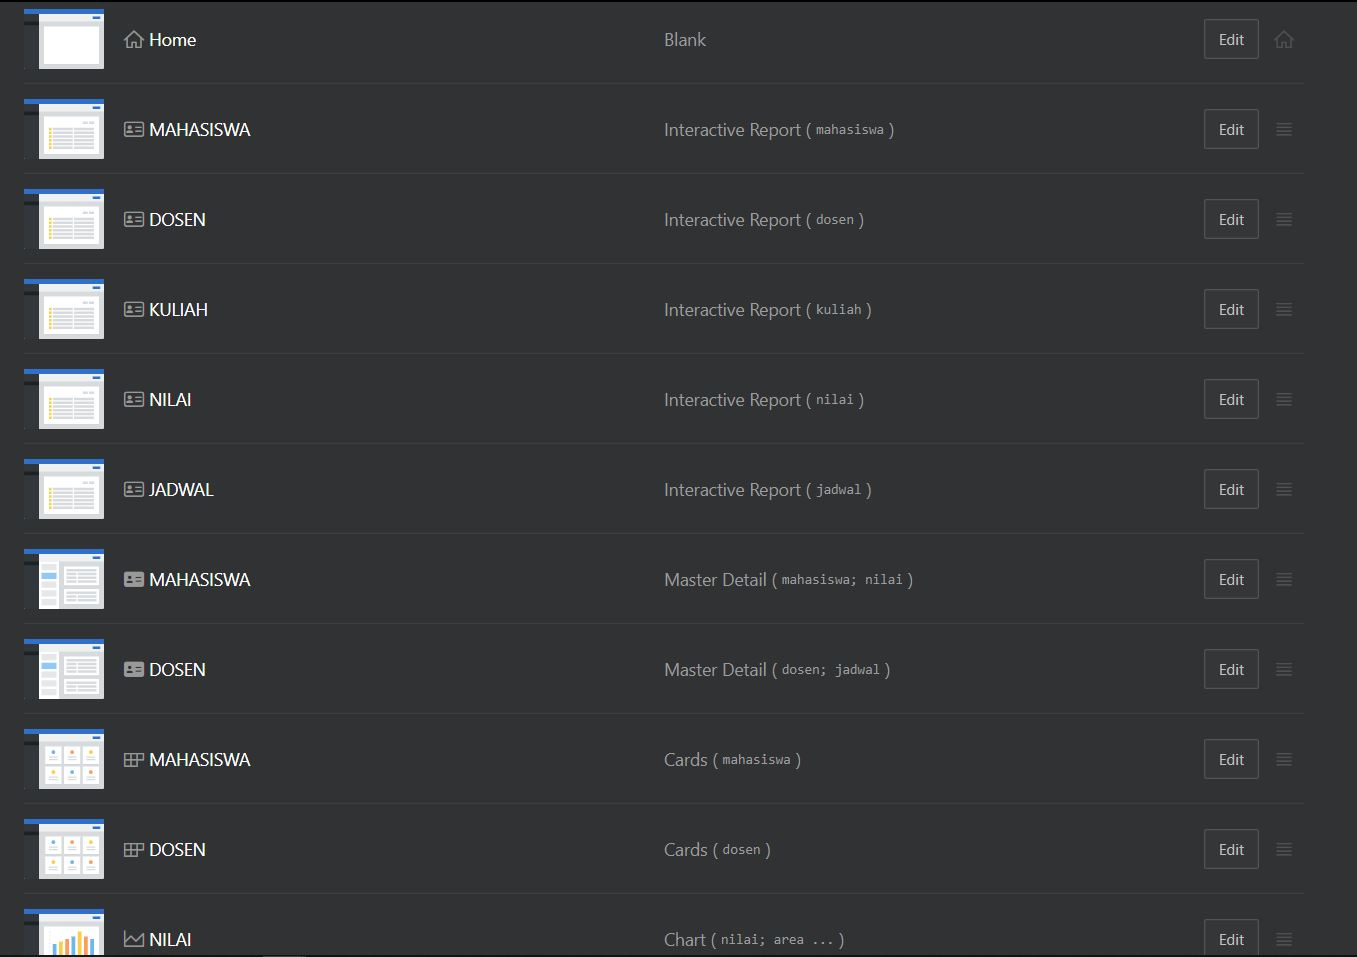
\includegraphics[scale=0.5]{section/ICA47.JPG}
    \caption{Tampilan Halaman Page yang telah dibuat}
    \end{center}   
    \end{figure} 
\item Langkah selanjutnya, create application setelah  selesai membuat fitur fiturnya
    \begin{figure}[!htbp]
    \begin{center}
    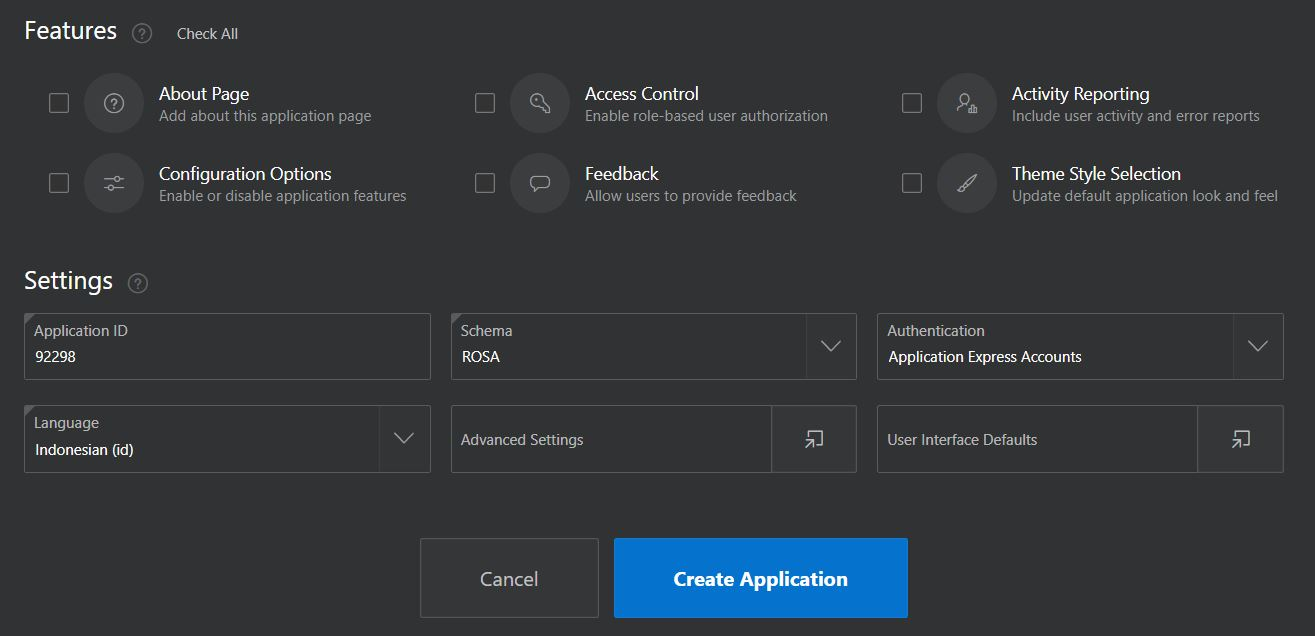
\includegraphics[scale=0.5]{section/ICA48.JPG}
    \caption{Tampilan Halaman Create Application}
    \end{center}   
    \end{figure} 
\item Kemudian kita Login menggunakan Email dan Password
    \begin{figure}[!htbp]
    \begin{center}
    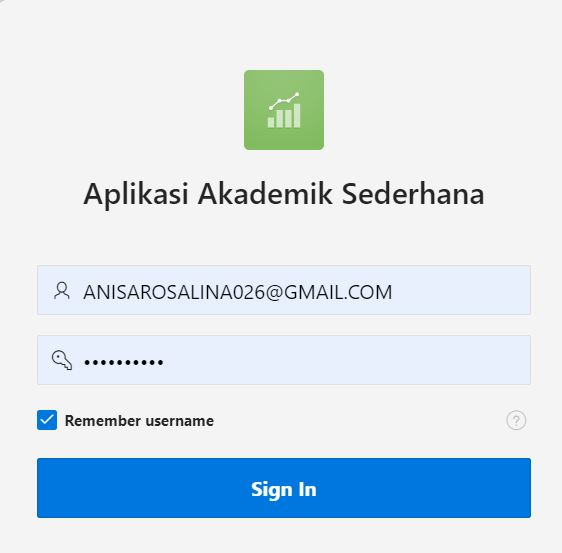
\includegraphics[scale=0.7]{section/ica50.JPG}
    \caption{Tampilan Halaman Login}
    \end{center}   
    \end{figure} 
\item Aplikasi Akademik Sederhana telah selesai kita buat.
    \begin{figure}[!htbp]
    \begin{center}
    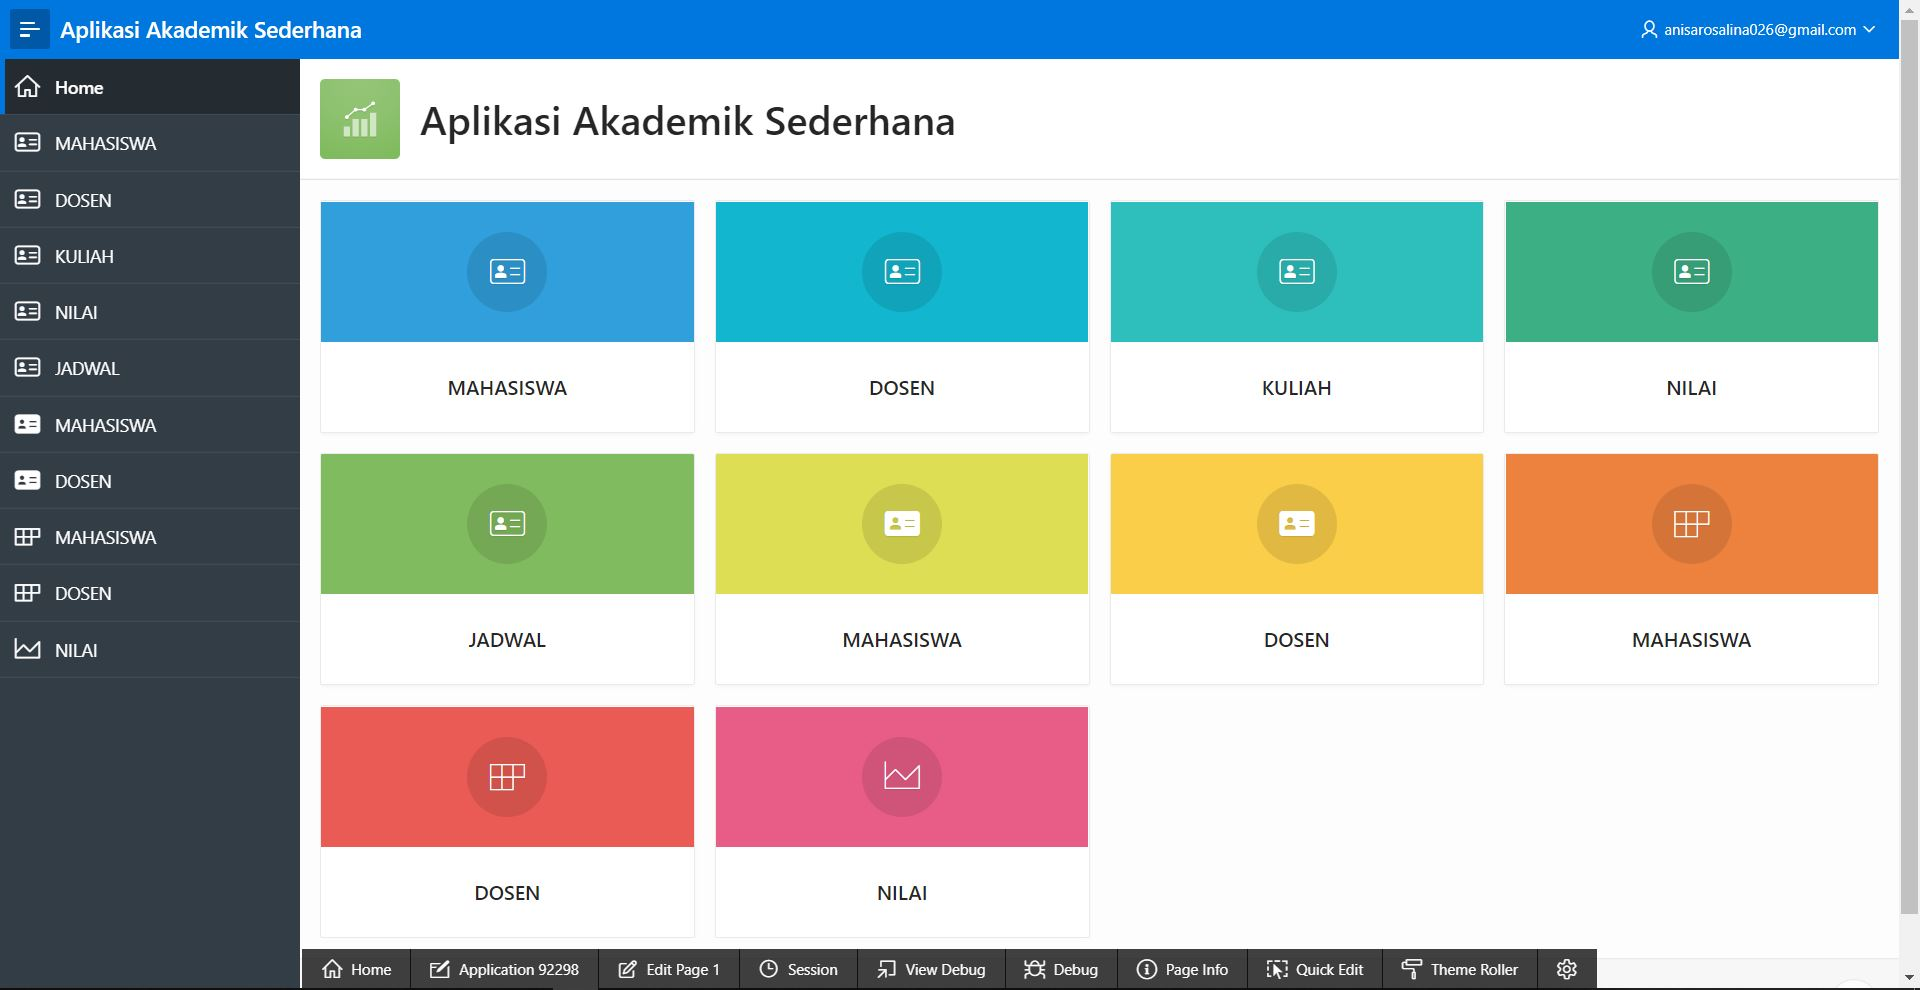
\includegraphics[scale=0.4]{section/ica61.JPG}
    \caption{Tampilan Home pada Aplikasi Akademik Sederhana}
    \end{center}   
    \end{figure} 
\item Tampilan Halaman Mahasiswa
    \begin{figure}[!htbp]
    \begin{center}
    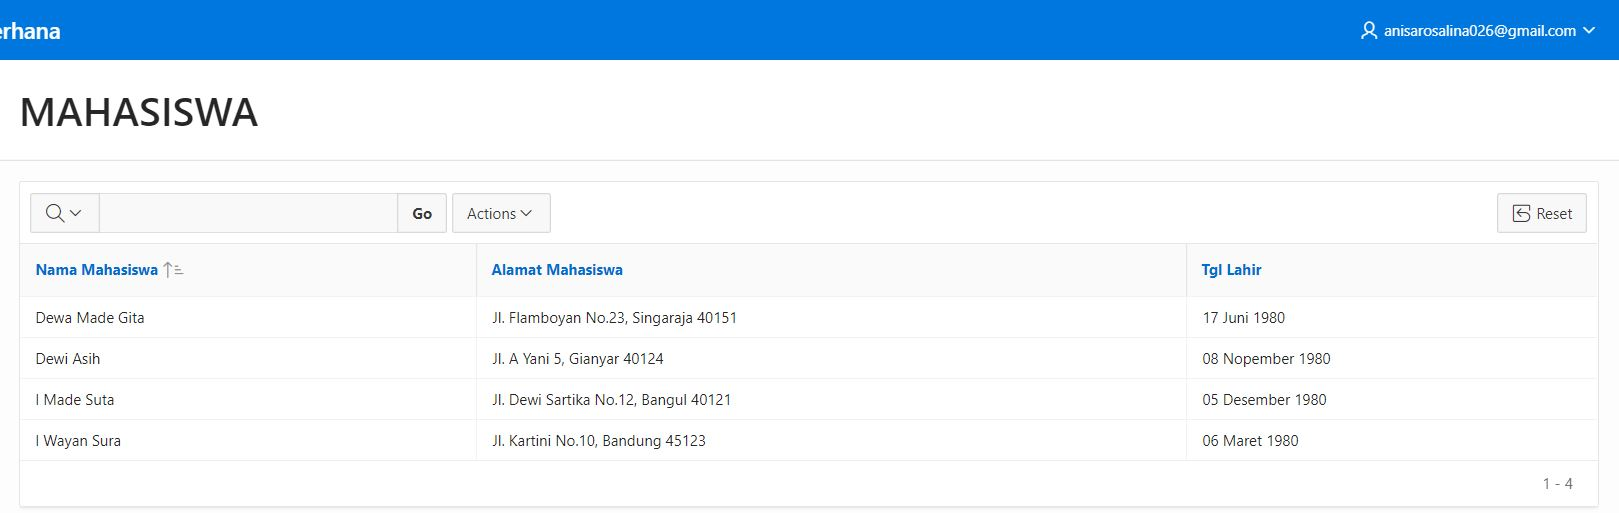
\includegraphics[scale=0.4]{section/ica63.JPG}
    \caption{Halaman Mahasiswa}
    \end{center}   
    \end{figure} 
\item Tampilan Halaman Dosen
    \begin{figure}[!htbp]
    \begin{center}
    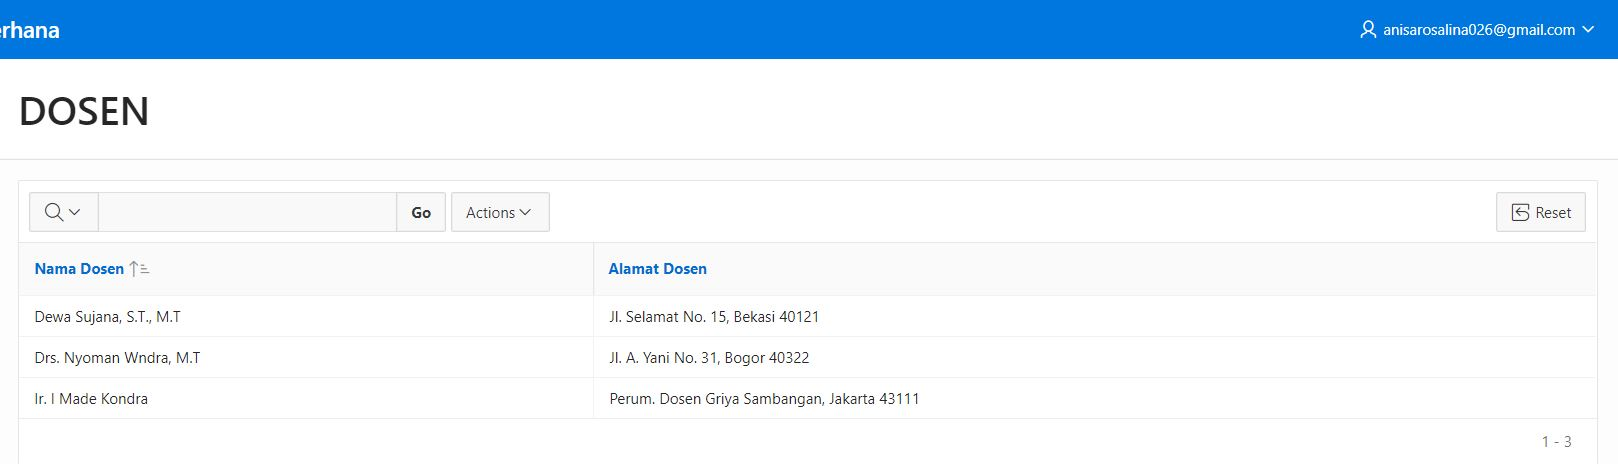
\includegraphics[scale=0.4]{section/ica64.JPG}
    \caption{Halaman Dosen}
    \end{center}   
    \end{figure} 
\item Tampilan Halaman Kuliah
    \begin{figure}[!htbp]
    \begin{center}
    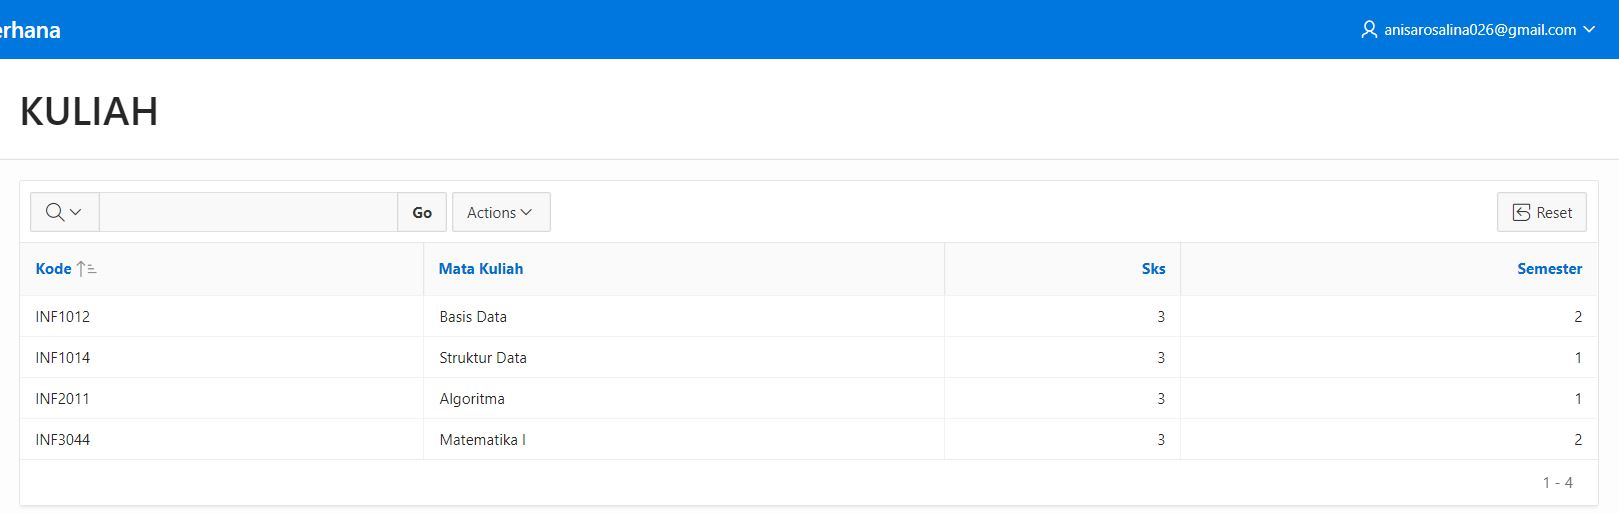
\includegraphics[scale=0.4]{section/ica65.JPG}
    \caption{Halaman Kuliah}
    \end{center}   
    \end{figure} \vspace{3cm}
\item Tampilan Halaman Nilai
    \begin{figure}[!htbp]
    \begin{center}
    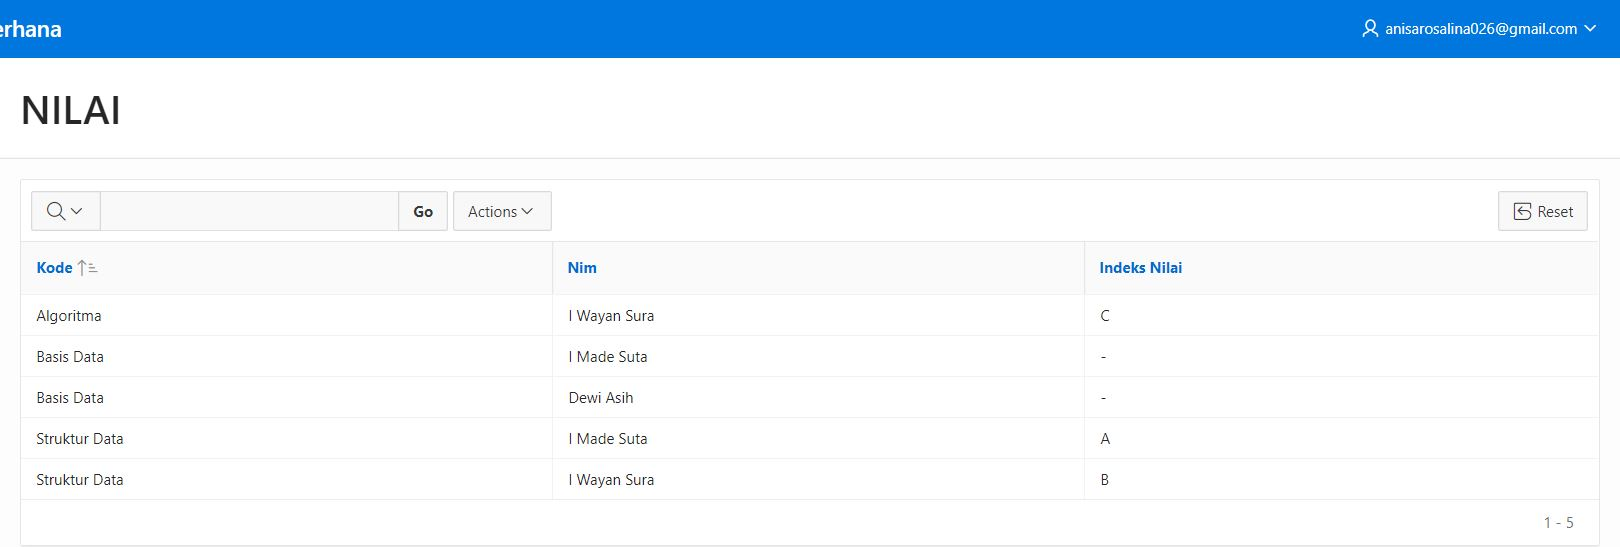
\includegraphics[scale=0.4]{section/ica66.JPG}
    \caption{Halaman Nilai}
    \end{center}   
    \end{figure} 
\item Tampilan Halaman Jadwal
    \begin{figure}[!htbp]
    \begin{center}
    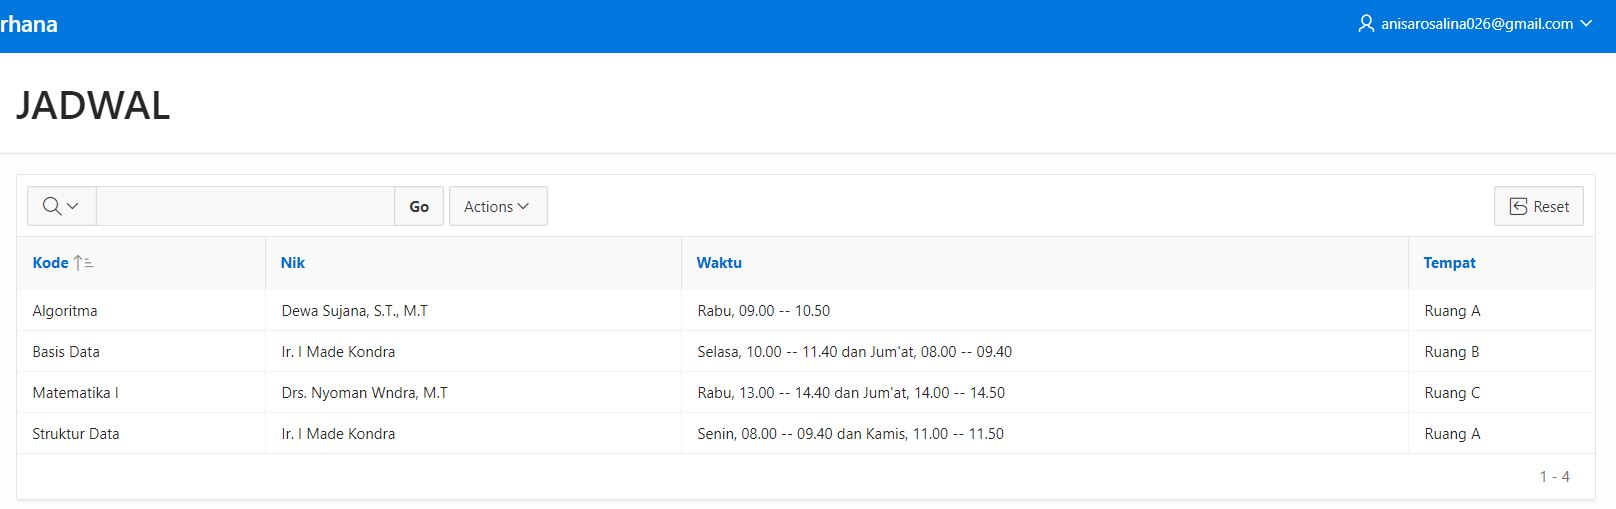
\includegraphics[scale=0.4]{section/ica67.JPG}
    \caption{Halaman Jadwal}
    \end{center}   
    \end{figure} 
\item Tampilan Halaman Cards Mahasiswa
    \begin{figure}[!htbp]
    \begin{center}
    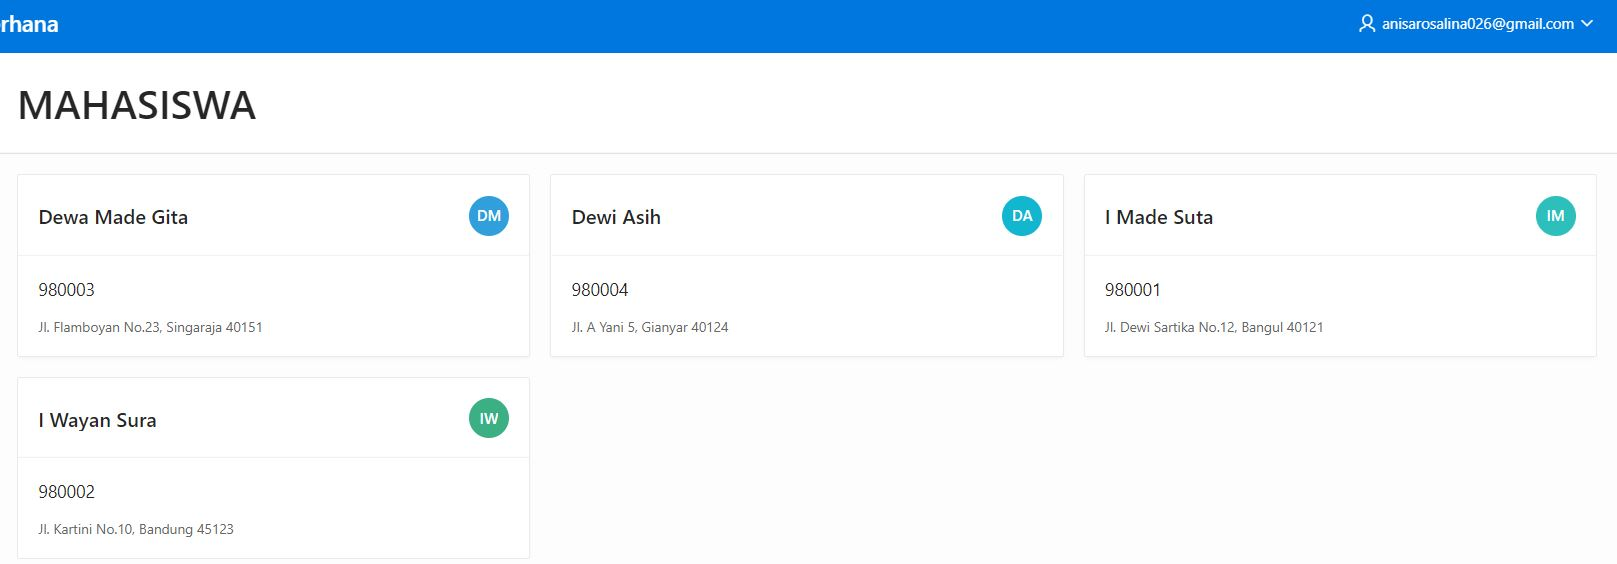
\includegraphics[scale=0.4]{section/ica68.JPG}
    \caption{Halaman Cards Mahasiswa}
    \end{center}   
    \end{figure} 
\item Tampilan Halaman Cards Dosen
    \begin{figure}[!htbp]
    \begin{center}
    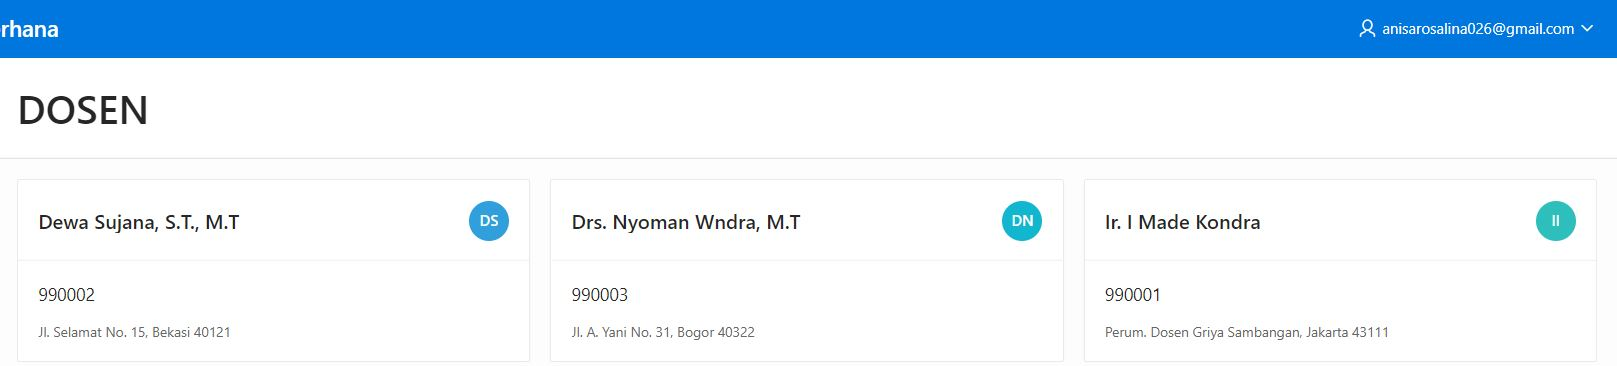
\includegraphics[scale=0.4]{section/ica69.JPG}
    \caption{Halaman Cards Dosen}
    \end{center}   
    \end{figure} 
\item Login Aplikasi  \\ https://apex.oracle.com/pls/apex/f?p=92298:14:715152119328418::NO::
\item Login Apex  \\    
Username        : ANISAROSALINA026@GMAIL.COM \\ Password        : anisa1184016
\end{enumerate}

